\section*{Materials and Methods}

\subsection*{Animals}

All experiments were conducted in adult transgenic mice (8--20 weeks) expressing either GCaMP6s or GCaMP8s in excitatory
cortical neurons under the CaMKII promoter. To enable simultaneous wide-field calcium imaging and optogenetic perturbation,
animals received a retro-orbital injection of a PHP-eB serotype adeno-associated viral (AAV) vector carrying a
DLX2.0-driven Chrimson construct, which restricts opsin expression to inhibitory interneurons and thereby enables focal
cortical suppression through inhibitory activation with minimal spectral cross-talk with GCaMP imaging. This dual-expression
configuration permitted mesoscale calcium measurement via GCaMP fluorescence and spatially localized, optogenetically
driven suppression within the same field of view. All procedures were approved by the Institutional Animal Care and Use
Committee (IACUC) at the University of Washington and were conducted in accordance with NIH guidelines for the care and use
of laboratory animals.

\subsection*{Surgical preparation and habituation}

A chronic trans-cranial window was implanted over the dorsal cortex to provide stable, long-term optical access to the
entire dorsal cortical surface in awake animals, following procedures described previously~\citep{Matveev2024}. Briefly,
the scalp and periosteum were removed and thin layers of UV-cured optical glue were applied to the exposed  skull surface inside a 3D-printed recording chamber secured with  dental cement, maintaining
transparency over the imaging field of view. A custom head-plate was attached to allow reproducible head-fixation across
sessions. Animals were allowed at least one week of recovery before any experimental handling.

\subsection*{Wide-field calcium imaging}

Neural activity was recorded using a custom single-photon mesoscopic fluorescence microscope with excitation and emission
filters matched to the GCaMP spectrum. Images were acquired at 70\,Hz with a 9.7\,mm $\times$ 9.7\,mm field of view, providing
mesoscale coverage of the entire dorsal cortical surface at a pixel resolution sufficient to resolve regional population
dynamics. Frames were collected using alternating blue (470\,nm) and violet (405\,nm) illumination at 35\,Hz per channel;
the violet channel captures hemodynamic absorbance and tissue auto fluorescence for correction purposes and was not used
for real-time computation. Light power was maintained below levels known to elicit photo toxicity or direct photo-stimulation of Chrimson.

Imaging data acquired for offline analysis were preprocessed using a standard pipeline including rigid motion correction,
reflectance normalization, and computation of $\Delta F/F$. Frames were registered to a common anatomical reference atlas,
and stimulation event timestamps were temporally aligned to the imaging data stream for trial-level analysis. Full
hardware specifications, surgical details, and viral constructs are described in~\citet{Matveev2024}.

\subsection*{Optogenetic stimulation}

Optogenetic stimulation was delivered concurrently with imaging via a secondary, spatially targeted illumination pathway
tuned to the Chrimson activation spectrum (638 nm). A galvanometer-steered laser beam was used to confine stimulation was used
to confine stimulation to a user-defined cortical region, specified as a two-dimensional coordinate relative to Bregma in
the control software. The stimulation target was positioned in a cortical region neighboring the $\Delta F/F$ output zone,
chosen such that the spatial spread of optogenetic activation encompassed the output region. Light power was calibrated
before each session using a power meter positioned at the objective focal plane. Stimulation pulse trains or constant-power
steps were delivered as analog voltage commands from a microcontroller, with a linear mapping between command voltage (0--5\,V)
and light power (0--36\,mW). Peak light power was capped at 36\,mW to remain within the unsaturated, physiologically safe
operating range of the opsin. Spectral separation between the GCaMP excitation band and the Chrimson activation band was
verified before each cohort of experiments; no measurable cross-talk was observed.

\subsection*{Real-time closed-loop system}

\subsubsection*{Hardware and software architecture}

The real-time experimental system was implemented in Python on a dedicated control server (CS). Wide-field images were
acquired using the Pylon image-capture API and streamed directly to the CS at 70\,Hz. Only blue-channel frames (35\,Hz
effective rate) were used for real-time computation; violet frames were discarded during online processing. The CS
displayed real-time images, $\Delta F/F$ traces, and experimental parameters via a graphical user interface (GUI). A
dedicated computation thread on the CS processed incoming frames, computed the feedback signal, evaluated the controller,
and transmitted stimulation commands to a microcontroller unit (MCU). The MCU performed digital-to-analog conversion and
drove the optogenetic stimulation hardware. A separate logging thread recorded all event timestamps---including image
acquisition triggers, controller outputs, and stimulation commands---to disk for offline analysis. The complete control
loop, from camera exposure trigger to stimulation command delivery, had a measured end-to-end latency of approximately
80\,ms (Figure~\ref{fig:system}B), arising from image transfer ($\sim$15\,ms), $\Delta F/F$ computation ($\sim$30\,ms),
and digital-to-analog conversion and stimulator settling ($\sim$35\,ms).

\subsubsection*{Online signal processing}

The real-time feedback signal was computed as the mean $\Delta F/F$ within a circular kernel centered on the designated
output region in somatosensory cortex. The $\Delta F/F$ signal was defined as
\begin{equation}
    y_t \;=\; \frac{F_t - \bar{F}}{|\bar{F}|},
    \label{eq:dff}
\end{equation}
where $F_t$ is the kernel-averaged fluorescence at frame $t$ and $\bar{F}$ is the running-window mean computed over a
preceding baseline window of fixed duration. The sign convention in the denominator ensures that $y_t$ correctly represents
fractional change even when $\bar{F}$ is negative, which can occur due to hemodynamic artifacts in uncorrected signals.
The $\Delta F/F$ trace was computed and visualized continuously on the GUI throughout the session.

\subsubsection*{Trial structure and experimental design}

Optogenetic stimulation was delivered in discrete trials of 3\,s duration, separated by 15\,s inter-trial intervals (ITIs)
during which no stimulation was applied and the animal rested. The reference signal was set to $y_{\mathrm{ref}} = -5\%\,\Delta F/F$
for the entire 3\,s stimulation window, corresponding to a target suppression of 5 percentage points relative to the running
baseline. Each session comprised 100 validation trials, of which half were randomly designated as closed-loop trials (feedback
active) and half as open-loop trials (feedforward only), interleaved in a pseudorandom order. This interleaving ensured that
the two conditions sampled the same distribution of brain states within each session. Each session began with a controller
tuning phase (see Section~\ref{sec:gain_opt}), after which the 100-trial validation block was initiated. Total experiment
duration was approximately 1\,h per session.

\subsection*{Mathematical framework}
\label{sec:math_framework}

\subsubsection*{Nonlinear system model}

The cortical response dynamics at the output region are modeled as a nonlinear, parameter-varying system driven by
optogenetic input:
\begin{align}
    x_{t+1} &= f(x_t,\, u_t,\, \rho_t) \;+\; d_t \;+\; w_t, \label{eq:nl_state}\\
    y_t     &= h(x_t,\, u_t,\, \rho_t) \;+\; v_t, \label{eq:nl_output}
\end{align}
where $x_t \in \mathbb{R}^n$ is the low-dimensional latent cortical state, $u_t \in \mathbb{R}$ is the scalar optogenetic
input, $\rho_t \in \mathbb{R}^p$ is a time-varying parameter vector encoding spontaneous brain-state fluctuations (e.g.\ 
arousal, movement, cortical synchrony), $d_t \in \mathbb{R}^n$ is an internal disturbance representing unobserved inputs
from other brain regions, $w_t \in \mathbb{R}^n$ is bounded process noise, $y_t \in \mathbb{R}$ is the measured
$\Delta F/F$ output at the output region, and $v_t \in \mathbb{R}$ is measurement noise. The functions $f$ and $h$ are
assumed continuous but otherwise unknown. The wide-field $\Delta F/F$ activity is biologically bounded, implying that the
system~\eqref{eq:nl_state}--\eqref{eq:nl_output} is marginally stable with oscillatory dynamics near a stationary mean. Here the state transition to the nonlinear dynamics at time $t$ can be written as 
\begin{align*}
    x(t) = \Phi(x_0,u,d,\rho) ; y(t)  = h\circ\Phi(x_0,u,d,\rho) 
\end{align*}
where $\Phi$ is the transition map. Here we assume that the initial condition $x_0$ is sampled from a set of feasible states, ie $x_0 \sim \mathcal{D}$. We assume that $x_0$ is drawn from the stationary distribution of the system with $\mathbb{E}[x_0] = \bar{x}_0$. Moreover, the disturbances $d$ and brain states $\rho$ are assumed to be sampled from a stationary distribution. By applying an input sequence $u_0,\ldots u_{t-1}$, we get a sample of the output trajectory $\mathcal{Y}_{0:T}$.    

\subsubsection*{Linear parameter-varying approximation}
\aditya{remove this argument if not necessary and supported by claims}
Because $f$ and $h$ are unknown and $\rho_t$ cannot be measured directly, exact nonlinear control is infeasible. We
instead consider a linear parameter-varying (LPV) approximation that captures the dominant input--output structure:
\begin{align}
    x_{t+1} &= A(\rho)\,x_t \;+\; B(\rho)\,u_t \;+\; w_t \;+\; d_t, \label{eq:lpv_state}\\
    y_t     &= C\,x_t \;+\; v_t, \label{eq:lpv_output}
\end{align}
where
\[
    A(\rho) \;=\; \sum_{k=1}^n \rho_k A_k, \qquad B(\rho) \;=\; \sum_{k=1}^n \rho_k B_k,
\]
and the parameter $\rho$ varies across trials due to spontaneous fluctuations in arousal, behavioral state, and network
dynamics. The disturbances $d_t$ and noise terms $w_t$, $v_t$ are assumed bounded and zero-mean. Because the distribution
of $\rho$ cannot be estimated reliably within experimental constraints, conventional system identification (frequency sweeps,
persistent excitation, subspace methods) is infeasible. Physiological constraints also limit the amplitude and duration of
permissible inputs, the number of trials per session, and total recording time. We therefore adopt a model-free approach to
controller design grounded in the following assumption.

\subsubsection*{Trial-averaging assumption}\label{sec:assumption1}
 
The output trajectory for time $t=0,1,\ldots, T$, for a given sequence of inputs $\mathcal{U}_{0:T-1} = u_0,u_1\ldots, u_{t-1}$, parametrized as $\mathcal{Y}_{0:T} = y_0,y_1,\ldots, y_T$ is generated by the nonlinear system Eq.(\ref{eq:nl_state}-\ref{eq:nl_output}). Here the initial condition was sampled from $\mathcal{D}$ and the disturbances and brain states were sampled from $P$ and $Q$ respectively. We hypothesize that the trial-averaged non-linear dynamics can be explained by a linear time-invariant(LTI) system, which requires no context of brain states or disturbances. Therefore, consider a LTI system:

\begin{align}
    x_{t+1} &= Ax_t + Bu_t \\
    y_{t} &= Cx_t \\
\end{align}

here the output trajectory can be written as $\bar{\mathcal{Y}}_{0:T} = \mathcal{A}x_0 + \Gamma \mathcal{U}_{0:T-1} $, where $\mathcal{A}$ and $\Gamma$ can be constructed from $A,B$ and $C$. We now state the trial-averaging assumption:


 
% \begin{align*}
% \bar{\mathcal{Y}}_{0:T} = 
%     \left[\begin{array}{c}
%          y_1  \\
%          y_2 \\
%          \vdots\\
%          y_T
%     \end{array}\right]  = \left[\begin{array}{c}
%          \bar{C}\bar{A}  \\
%          \bar{C}\bar{A}^2 \\
%          \vdots\\
%          \bar{C}\bar{A}^{T-1}
%     \end{array}\right]\bar{x}_0 + \left[\begin{array}{cccc}
%          \bar{C}\bar{B} & \times &\ldots & \times \\
%          \bar{C}\bar{A}\bar{B} & \bar{C}\bar{B} & & \vdots \\
%          \vdots&&&\times\\
%          \bar{C}\bar{A}^{T-1}\bar{B} &\ldots& \bar{C}\bar{A}\bar{B}& \bar{C}\bar{B}   \\
%     \end{array}\right]\left[\begin{array}{c}
%          u_0  \\
%          u_1 \\
%          \vdots\\
%          u_{T-1}
%     \end{array}\right]
% \end{align*}


% \begin{assumption} (\textbf{Trial-Averaging}) 
% \label{as:averaging}
% The trial-averaged system response can be well-approximated by a stationary linear system:
% \[
% \mathbb{E}[{\mathcal{Y}}_{0:T}(x_0,u_{0:T-1},\rho_{0:T-1},d_{0:T-1})] = \bar{\mathcal{Y}}_{0:T},
% \]    \label{eq:assumption1}
% where $\bar{\Sigma}$ is the output sequence generated by the nominal linear system $(\bar{A}, \bar{B}, C)$ with $d_t = 0$ and $\mathbb{E}[x_0] = \bar{x}_0$. The parameters $\rho \in P$ and disturbances $d \in Q$ are drawn from bounded, stationary sets.
% \end{assumption}
% \subsubsection{Trial-averaging assumption}
% \label{sec:assumption1}

\medskip
\noindent\textbf{Assumption 1} (Trial-averaging). \textit{The trial-averaged output sequence of the nonlinear system~\eqref{eq:nl_state}--\eqref{eq:nl_output} is well approximated by  he output sequence of a nominal linear time-invariant (LTI) system $({A}, {B}, C)$ with zero disturbance and zero-mean noise:}
\begin{equation}
    \mathbb{E}\!\left[\mathcal{Y}_{0:T}(x_0,u, d, \rho)\right]
    \;=\;
    \bar{\mathcal{Y}}_{0:T}(x_0,u),
    \label{eq:assumption1}
\end{equation}
\textit{where $\mathcal{Y}_{0:T}$ denotes the output trajectory of the nonlinear system initiated at $x_0$, $\bar{\mathcal{Y}}_{0:T}$ denotes the output trajectory of the nominal LTI system initiated at
$\bar{x}_0 = \mathbb{E}[x_0]$ The parameter $\rho \in \mathcal{P}$ and disturbances $d \in \mathcal{Q}$ are
drawn from bounded, stationary sets, such that $\mathbb{E}[d_t] = 0$ and $\mathbb{E}[\rho_t] = \bar{\rho}$ hold
approximately over the session.}
\medskip


% \begin{figure}
%     \centering
%     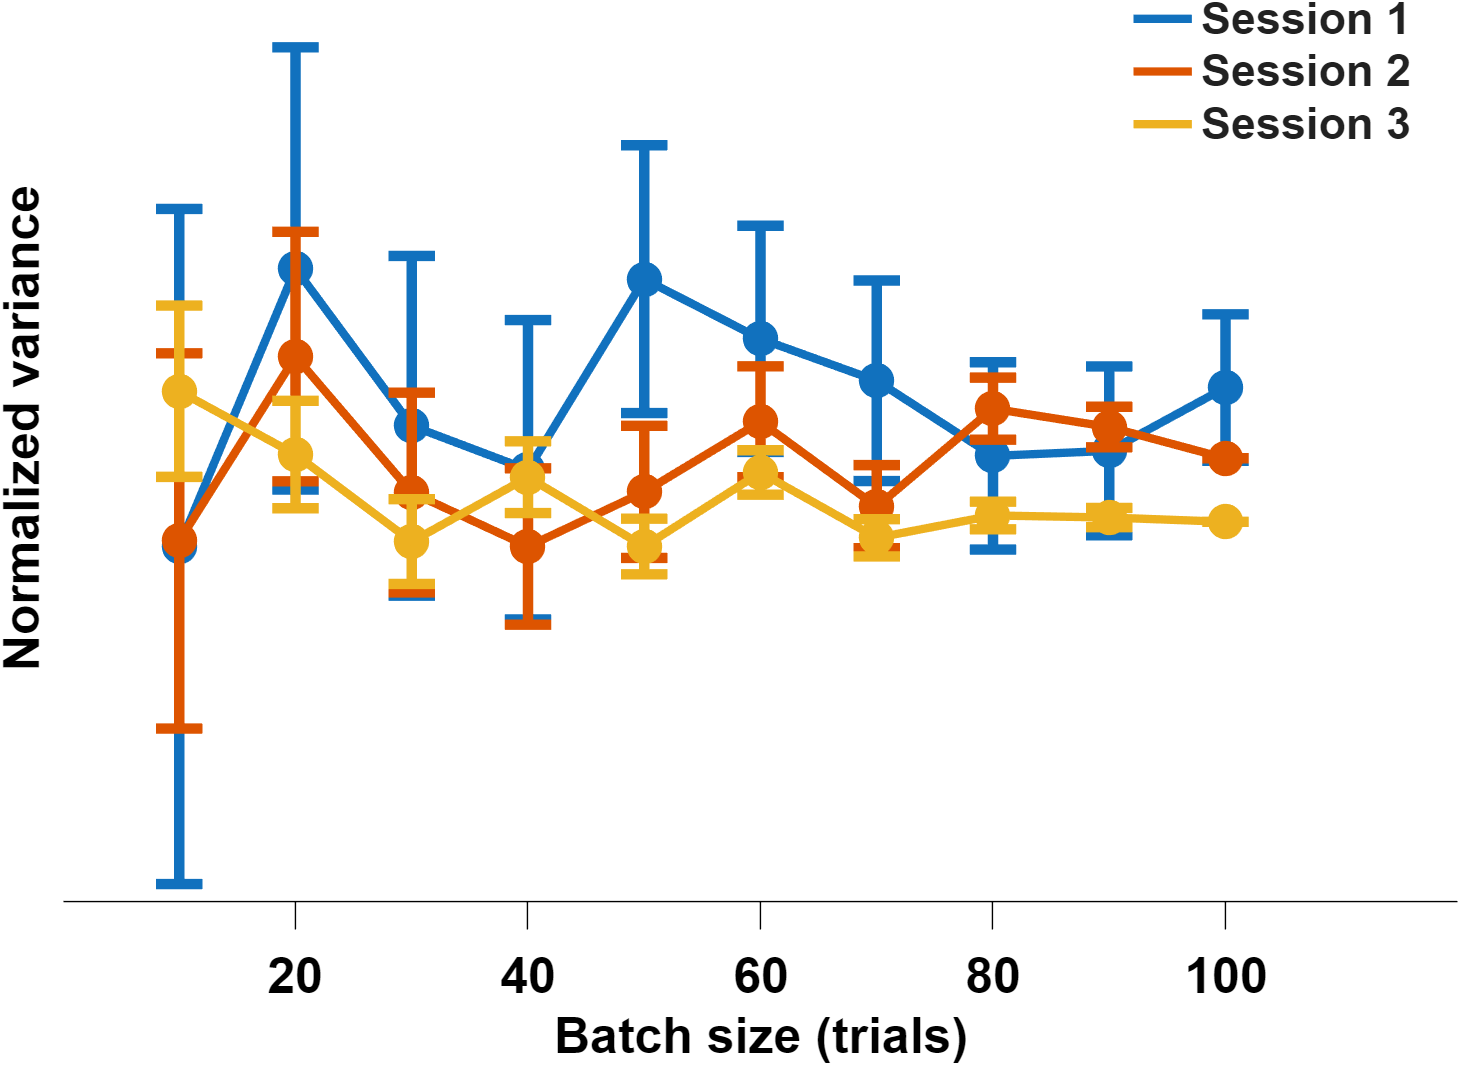
\includegraphics[width=0.5\linewidth]{images/spont_variance.png}
%     \caption{ Total variance as a function of trial batch size across experiment sessions}
%     \label{fig:variance_batch}
% \end{figure}

Under Assumption~\ref{sec:assumption1}, trial-to-trial deviations from the averaged response are due to zero-mean
perturbations that cancel in expectation. The nominal system $(\bar{A}, \bar{B}, C)$ therefore provides the effective
input--output model on which the controller is designed. Empirical support for this assumption is provided by analyzing variance of trials across various batch sizes in an experiment as shown in Figure~\ref{fig:variance_batch}).

\subsection*{System characterization}
\label{sec:system_char}

\subsubsection*{Impulse response protocol}

To assess the linearity and monotonicity of the input--output relationship, impulse-like optogenetic inputs were delivered
at varying amplitudes sampled from a discrete set (0, 0.8, 1.6, 2.4, 2.7\,V). Trials were interleaved with randomized
inter-trial intervals and delivered in pseudo-random amplitude order. The response to each amplitude level was quantified as
the mean peak $\%\,\Delta F/F$ suppression across trials, where peak timing was determined from the trial-averaged waveform
at the highest stimulus amplitude. A linear regression of peak suppression on stimulus amplitude was used to assess
input--output linearity and to estimate the feedforward gain $K_r$ (see Section~\ref{sec:feedforward}). A minimum of 20
trials per amplitude level was required for inclusion in the linear fit.

\subsubsection*{Step response protocol}

To characterize steady-state dynamics and estimate the effective gain of a sustained stimulus, a constant optogenetic input
was applied at a fixed voltage for 3\,s trial windows, with trials spaced by a fixed ITI across the session. The
trial-averaged step response was compared to its within-window mean as a proxy for steady-state output. Variance across
trials was also computed as a function of time to assess the stability of the response and the validity of
Assumption~\ref{sec:assumption1} across sessions.

% \subsubsection{Brain-state analysis}

% To assess the dependence of input--output linearity on cortical state, the power spectral density of the pre-stimulus
% $\Delta F/F$ signal (0.5\,s window) was computed on each trial, and total power in the low-frequency band ($<2$\,Hz)
% was used as a proxy for cortical synchrony~\citep{Harris2011}. Trials were median-split into low-power (desynchronized)
% and high-power (synchronized) subsets. Impulse response peak suppression was then compared across subsets to determine
% whether the monotonic input--output relationship depended on brain state.

\subsection*{Controller design}

\subsubsection*{Feedforward gain calibration}
\label{sec:feedforward}

The feedforward component of the controller provides the nominal input required to achieve an output close to
$y_{\mathrm{ref}}$, compensating for the baseline gain of the optogenetic actuator. The feedforward command at each
timestep is:
\begin{equation}
    \bar{u}_t \;=\; K_r\!\left(y_{\mathrm{ref}} - y_t\right),
    \label{eq:feedforward}
\end{equation}
where $K_r$ is a scalar gain estimated from the impulse response calibration experiment. Let
$U = [u_1, \ldots, u_K] \in \mathbb{R}^{1 \times K}$ be the row vector of stimulus amplitudes and
$Y = [(y_1 - y_{\mathrm{ref}}), \ldots, (y_K - y_{\mathrm{ref}})] \in \mathbb{R}^{1 \times K}$ the corresponding
trial-averaged output deviations from the reference. The least-squares feedforward gain is:
\begin{equation}
    K_r \;=\; U Y^\dagger,
    \label{eq:Kr}
\end{equation}
where $Y^\dagger$ denotes the Moore--Penrose pseudoinverse. This estimate provides an approximate open-loop
inversion of the input--output map and serves as the baseline for PI feedback augmentation.

\subsubsection*{Proportional--integral feedback controller}
\label{sec:pi_controller}

To compensate for model bias in $K_r$, residual nonlinearities, trial-to-trial disturbances, and brain-state-dependent
deviations that the feedforward term cannot correct, a proportional--integral (PI) feedback controller is appended to
the feedforward command. The total stimulation input at each timestep is:
\begin{equation}
    u_t \;=\; K_r\!\left(y_{\mathrm{ref}} - y_t\right)
             \;+\;
             K_p\!\left(y_{\mathrm{ref}} - y_t\right)
             \;+\;
             K_i \sum_{k=0}^{t}\!\left(y_{\mathrm{ref}} - y_k\right)\Delta t,
    \label{eq:controller}
\end{equation}
where $K_p > 0$ is the proportional gain and $K_i > 0$ is the integral gain. The proportional term provides
timestep-level correction proportional to the instantaneous tracking error; the integral term accumulates signed
error across the trial to eliminate persistent bias. Anti-windup clamping was applied to the integral accumulator to
prevent integrator saturation during periods when the actuator is saturated. The command $u_t$ was clipped to the
feasible range $[0,\, 5\,\text{V}]$ before transmission to the optogenetic stimulator, corresponding to a maximum
light power of 36\,mW.

In the open-loop condition, feedback gains were set to $K_p = K_i = 0$, reducing~\eqref{eq:controller} to the
feedforward term~\eqref{eq:feedforward} alone. This provides the comparison baseline against which closed-loop
performance is evaluated.

\subsubsection*{Augmented state representation}

To facilitate analysis of the closed-loop system with linearity assumption on the trial averages system, the integral action in~\eqref{eq:controller} is represented as an augmented state variable $\xi_t = \sum_{k=0}^{t}(x_k - x_{\mathrm{ref}})\,\Delta t$. The augmented state vector
$s_t = [x_t^\top,\, \xi_t^\top]^\top$ satisfies:
\begin{equation}
    \begin{bmatrix} x_{t+1} \\ \xi_{t+1} \end{bmatrix}
    \;=\;
    \begin{bmatrix} \bar{A} & 0 \\ I\,\Delta t & I \end{bmatrix}
    \begin{bmatrix} x_t \\ \xi_t \end{bmatrix}
    \;+\;
    \begin{bmatrix} \bar{B} \\ 0 \end{bmatrix} u_t,
    \label{eq:aug_state}
\end{equation}
\begin{equation}
    y_t \;=\; \begin{bmatrix} C & 0 \end{bmatrix} s_t,
    \label{eq:aug_output}
\end{equation}
and the feedback control law takes the compact form $u_t = K s_t$, where $K = [K_p,\, K_i]$.
Under Assumption~\ref{sec:assumption1}, the closed-loop system~\eqref{eq:aug_state}--\eqref{eq:aug_output} with
$u_t = Ks_t$ is stable provided the proportional gain is consistent with the approximately monotonic input--output
relationship established empirically~\citep{Astrom1995}.

\subsection*{Controller gain optimization}
\label{sec:gain_opt}

\subsubsection*{Performance metric}

Controller performance was quantified using the mean-squared tracking error accumulated over each trial. The per-trial
tracking cost for an experiment initiated at latent state $x_0$ under gain $K$ is:
\begin{equation}
    c(x_0;\, K) \;=\; \sum_{t=0}^{T} \bigl\|z(t)\bigr\|^2,
    \qquad z(t) \;=\; y_t - y_{\mathrm{ref}},
    \label{eq:trial_cost}
\end{equation}
and the expected cost over the distribution $\mathcal{D}$ of initial conditions and brain states is:
\begin{equation}
    J(K) \;=\; \mathbb{E}_{x_0 \sim \mathcal{D}}\!\left[c(x_0;\, K) \;\middle|\; K\right].
    \label{eq:expected_cost}
\end{equation}
In practice, $J(K)$ is estimated by the Monte Carlo approximation:
\begin{equation}
    \hat{J}(K) \;=\; \frac{1}{N}\sum_{i=1}^{N}\sum_{t=0}^{T}
                     \bigl\|z_i(t)\bigr\|^2,
    \label{eq:emp_cost}
\end{equation}
where the $N$ trials provide independent samples of $c(x_0;\, K)$. Under Assumption~\ref{sec:assumption1},
$\hat{J}(K) \to J(K)$ as $N \to \infty$. The approximation error (regret) is:
\begin{equation}
    R(N,\, K) \;=\; \hat{J}(K) - J(K),
    \label{eq:regret}
\end{equation}
which decreases at rate $O(1/\sqrt{N})$ for independent, identically distributed trials. In practice, $R(N, K)$ can
be inflated by brain-state non-stationarity across the session (see Discussion).

\subsubsection*{Zeroth-order gain search}
\label{sec:zeroth_order}


\begin{figure}[!ht]
    \centering

  \begin{subfigure}[t]{0.6\linewidth}
        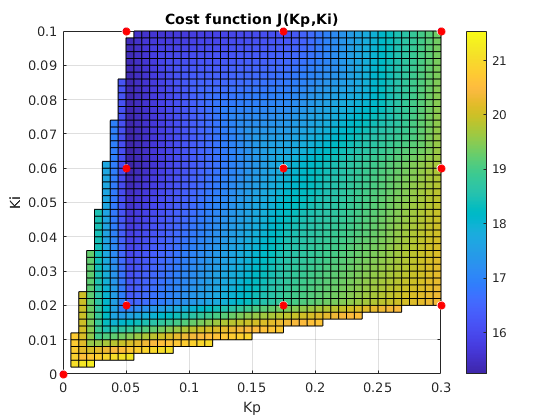
\includegraphics[width=\linewidth]{images/jval_controllers2503051.png} 
        \caption*{\textbf{A}}
    \end{subfigure}
    
    % ---------- Panel C: Controller performance landscape ----------
    \begin{subfigure}[t]{\linewidth}
    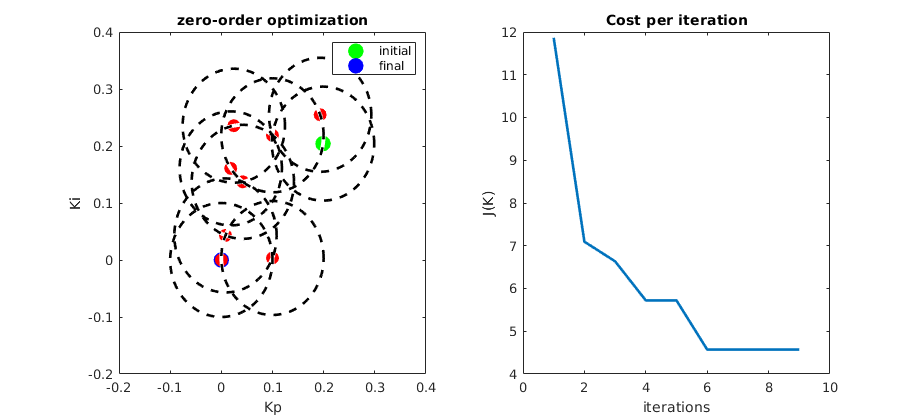
\includegraphics[width=\linewidth]{images/opt.png}
    \caption*{\textbf{B}}
    \end{subfigure}

    \caption{
        \textbf{Closed-loop controller performance metrics.}
        (\textbf{A})Empirical performance landscape of candidate controllers, showing the trial-averaged tracking cost $J(K)$ as a function of controller gains, used to guide zero-order controller optimization for a single session.
        (\textbf{B-C}) Model-free optimization of the controller using the zero-order search routine in Algorithm~\ref{alg:zeroopt}. Each point represents the tracking cost $\hat{J}(K)$ for a candidate controller, and the trajectory shows the evolution of controller gains during the experiment.}
    \label{fig:cost_landscape}
\end{figure}


Direct gradient-based optimization of $J(K)$ is infeasible because gradients cannot be computed analytically without an
explicit system model, and because the number of trials required to estimate $J(K)$ accurately is limited by experimental
constraints. Instead, we map the empirical cost landscape over a grid of candidate gains
$K \in [0, 0.3] \times [0, 0.1]$ (Figure~\ref{fig:cost_landscape}A), then refine using a model-free zeroth-order
search (Algorithm~\ref{alg:zeroth_order}).

\begin{algorithm}[h]
\caption{Zeroth-order controller gain search}
\label{alg:zeroth_order}
\begin{algorithmic}[1]
\State \textbf{Initialize:} gain $K_0 = [K_p^{(0)},\, K_i^{(0)}]$, step size $r$
\For{$i = 1$ \textbf{to} $I$}
    \State Sample $\mathbf{v}$ uniformly from the unit 2-sphere
    \State Propose $K_i \leftarrow K_{i-1} + r\,\mathbf{v}$
    \For{$j = 1$ \textbf{to} $N$}
        \State Run one trial of length $T$ under controller $K_i$
        \State Compute $C_j = \sum_{t=0}^{T} \|z_j(t)\|^2$
    \EndFor
    \State Compute $\hat{J}(K_i) = \frac{1}{N}\sum_{j=1}^{N} C_j$
    \If{$\hat{J}(K_i) \geq \hat{J}(K_{i-1})$}
        \State $K_i \leftarrow K_{i-1}$ \Comment{Reject update}
        \State $r \leftarrow r / 2$ \Comment{Shrink step size}
    \EndIf
\EndFor
\end{algorithmic}
\end{algorithm}

The algorithm accepts a new gain vector only when it strictly reduces $\hat{J}$; otherwise the current gain is retained
and the search radius is halved. The optimization was initialized with $K_0$ set to the best-performing gain from the
grid sweep (Figure~\ref{fig:cost_landscape}B). A controller was considered acceptable if $\hat{J}(K) \leq \hat{J}(\mathbf{0})$,
where $\hat{J}(\mathbf{0})$ is the empirical cost of the open-loop (feedforward-only) controller, ensuring that feedback
control was validated to improve upon the open-loop baseline before the validation block commenced.

\subsection*{Disturbance attribution analysis}
\label{sec:disturbance}

To identify the sources of residual trial-to-trial tracking error, we related the per-trial open- and
closed-loop tracking error to concurrent movement and to pre-stimulus cortical state.

\subsubsection*{Per-trial tracking error}

For each trial, tracking error was quantified as the root-mean-squared deviation of the output $y_t$ from the
reference $y_{\mathrm{ref}}$ over the window $t = +1$ to $+3$\,s relative to laser onset; the initial
$0$--$1$\,s interval was excluded so that the metric captured steady-state regulation rather than the
inhibitory onset transient. Per-trial error was z-scored within each session to permit pooling across
sessions, and high-error trials were defined as the top quartile of the within-session error distribution.

\subsubsection*{Movement disturbance}

Concurrent movement was quantified from a simultaneously acquired behavioral video as a per-trial
motion-energy scalar, averaged over the trial window and z-scored within session. For each session with
simultaneous motion capture ($n = 9$), z-scored per-trial motion energy was regressed on z-scored tracking
error separately for open- and closed-loop trials, and the resulting slopes were compared between conditions
using the Wilcoxon signed-rank test. Trials with z-scored motion energy exceeding $1.5$ were classified as
high-motion and excluded from the spectral analysis below.

\subsubsection*{Low-frequency spontaneous fluctuations}

To isolate the contribution of spontaneous cortical activity from movement, the spectral analysis was
restricted to motion-clean trials (z-scored motion energy $\leq 1.5$). For each retained trial, the power
spectrum of the $\Delta F/F$ output was estimated in $0.5$\,Hz bins spanning $0$--$10$\,Hz, and the
\emph{low-frequency power} was defined as the integrated absolute power in the $1$--$4$\,Hz band over the
pre-stimulus interval preceding laser onset. Absolute power ($(\Delta F/F)^2\,\mathrm{Hz}^{-1}$) was used
throughout, without normalization or z-scoring of the spectra. We then quantified the fraction of high-error
closed-loop trials (top error quartile) that coincided with elevated pre-stimulus low-frequency power, to
estimate the share of residual closed-loop tracking error attributable to low-frequency spontaneous
fluctuations rather than to movement. Representative low- and high-error single-trial spectra are reported as
a supplementary figure (Figure~S\ref{fig:lowfreq_examples}).

\section*{Supplementary Data}

\subsection*{Statistical analysis}

No formal statistical tests were pre-registered for this study. Comparisons between open-loop and closed-loop conditions
were made using the empirical per-trial cost $\hat{J}(K)$ defined in Equation~\eqref{eq:emp_cost}. Session-averaged
performance was summarized using mean and standard deviation across trials. Variance in cortical activity was computed
as the sample variance of $y_t$ across trials at each timestep within the stimulation window. Batch-size convergence
(Figure~\ref{fig:variance_batch}) was assessed by computing the mean total variance $\mathrm{Var}(y_t)$ as a function
of increasing batch size $N$, averaged over five independent subsamples per batch size.

\clearpage
\setcounter{figure}{0}
\renewcommand{\thefigure}{S\arabic{figure}}


\begin{figure}
    \centering
    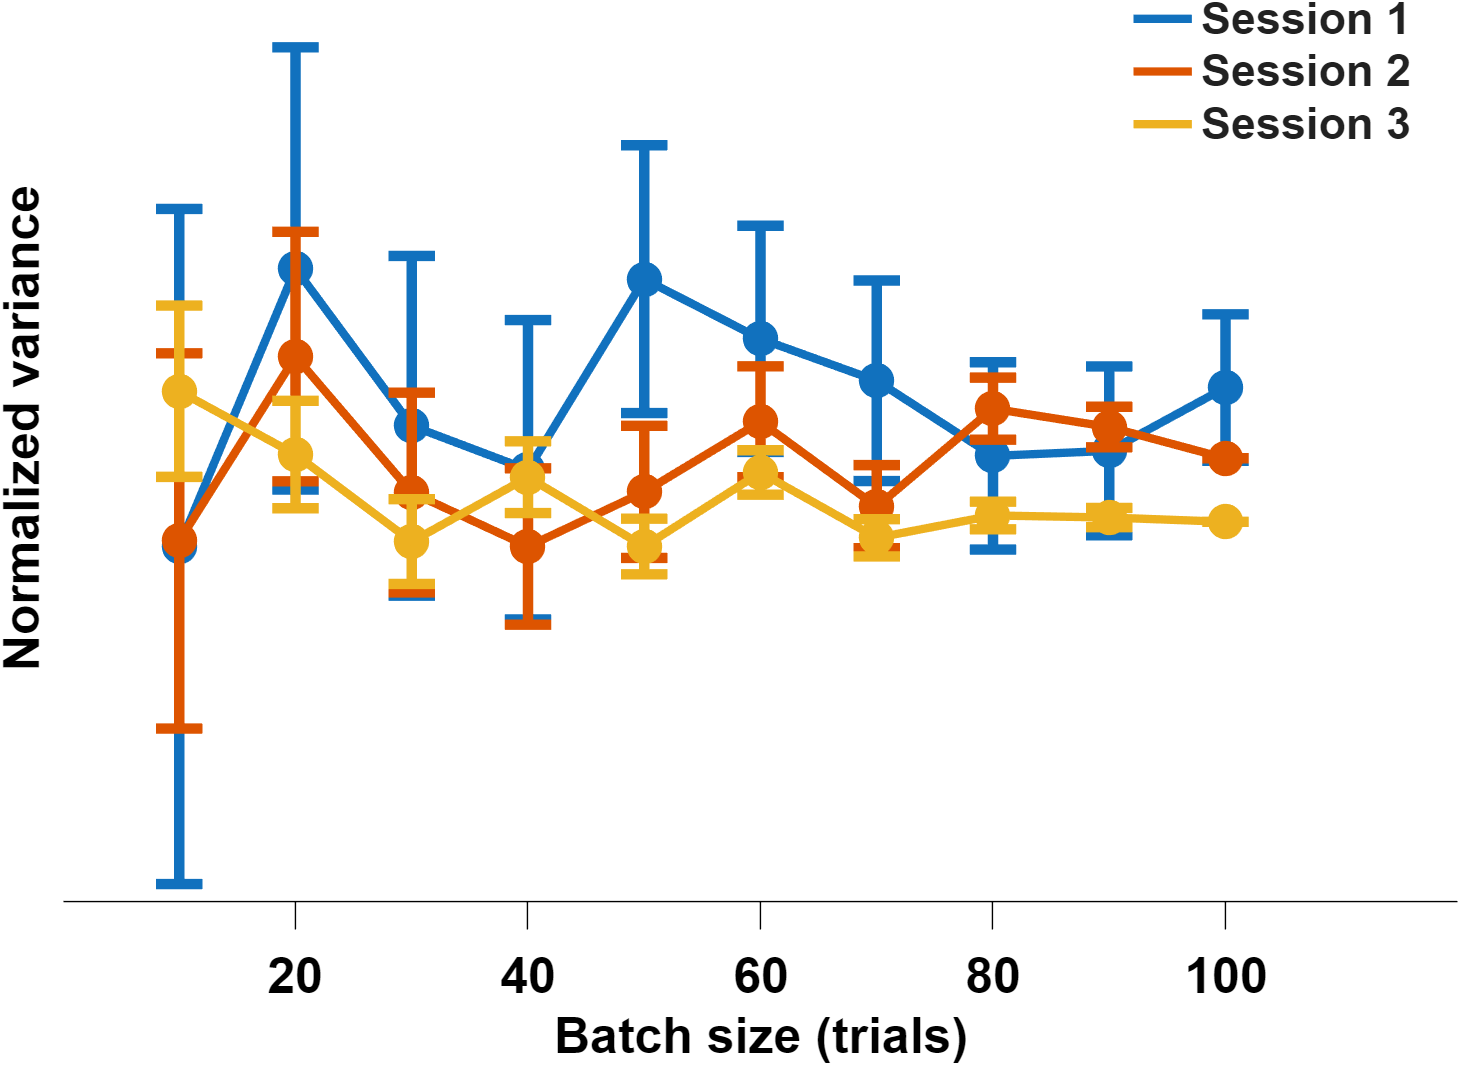
\includegraphics[width=0.5\linewidth]{images/spont_variance.png}
    \caption{Total variance as a function of trial batch size across experiment sessions}
    \label{fig:variance_batch}
\end{figure}

% PLACEHOLDER -- representative low-frequency spectral examples (AL to select trials/sessions).
% Drop the chosen good-/bad-trial spectra into images/lowfreq_examples.* and remove the TODO note.
\begin{figure}
    \centering
    % \includegraphics[width=0.7\linewidth]{images/lowfreq_examples.pdf}
    \todo{Representative single-trial spectra: a low-error and a high-error motion-clean closed-loop trial,
    showing pre-stimulus $\Delta F/F$ power $(\Delta F/F)^2$/Hz with the $1$--$4$\,Hz low-frequency band
    highlighted. Example trials to be selected by AL.}
    \caption{Representative pre-stimulus power spectra for a low-error and a high-error motion-clean
    closed-loop trial. Low-frequency ($1$--$4$\,Hz) power is elevated on the high-error trial.}
    \label{fig:lowfreq_examples}
\end{figure}